\documentclass{standalone}
\usepackage{tikz}

\begin{document}

  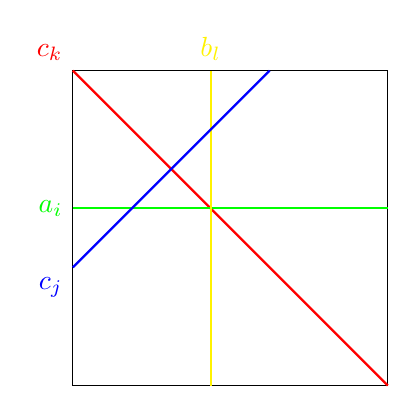
\begin{tikzpicture}[scale= 0.5,>=latex]
    \draw (0,0) rectangle (8,8);
    \draw[thick,red](0,8)node[above left]{$c_k$}--(8,0);
    \draw[thick,green](0,4.5)node[left]{$a_i$}--++(8,0);
    \draw [thick,yellow](3.5,0)--++(0,8)node[above]{$b_l$};
    \draw[thick,blue](0,3)node[below left]{$c_j$}--++(5,5);
  \end{tikzpicture}

\end{document}
